% Title page
\thispagestyle{fancy}
\fancyhf{}
\lfoot{Date: \hspace{15em} Signature:}
\renewcommand{\footrulewidth}{0pt}

\vspace*{6em}
\fontfamily{phv}\selectfont
\begin{center}
    \begingroup
    \fontsize{60}{30}
    \textcolor{ThesisColor}{\textbf{Thesis}}\\
    \vspace{6em}
    \textbf{\Huge \ThesisName\\}
    \endgroup 
    
\includegraphics[scale=0.4]{assets/logo.png}\\
    \renewcommand{\arraystretch}{2}
    \setlength{\tabcolsep}{10pt}
    \begin{tabular}{c c c}
        \textbf{Performed by} & \textbf{Year/Grade} & \textbf{Supervisor}\\
        Tobias Haubenwallner & 2021/2022 5BHET & Prof. DI Christoph Wurzinger
    \end{tabular}
\end{center}
\vspace{8.5em}
\newpage
\pagestyle{fancy}
\fancyhf{}
\renewcommand{\headrulewidth}{0pt}
\renewcommand{\footrulewidth}{0pt}
\fancyfoot[L]{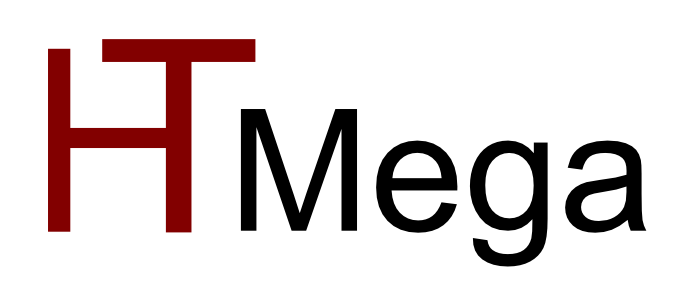
\includegraphics[height=3em, valign=c]{assets/logo-small.png}}
\fancyfoot[R]{\thepage \: of \pageref{LastPage}}



% Declaration of Honour
\section*{Declaration of Honor}
\addcontentsline{toc}{section}{Declaration of Honour}

I hereby declare, that I wrote the present thesis for myself and without foreign help.\\
Furthermore, I have not used sources and aid other than those stated.
\vspace{6em}\\
Date: \hspace{15em} Signature:
\newpage


% Brief Description
\section*{Abstract}
\addcontentsline{toc}{section}{Abstract}
The goal of this thesis is to develop and create a custom and functional microcontroller on an FPGA.

\subsection*{Functionality \& Features}
\addcontentsline{toc}{subsection}{Features}

\paragraph{Core Device Functionalities}
\begin{itemize}
    \item Functional 16-bit 6 MHz computation machine consisting of CPU and memory in harvard architecture
    \item Implemented Turing complete instruction set
\end{itemize}

\paragraph{Additional Device Features}
\begin{itemize}
    \item Bootloader enabling programming over a USB connector
    \item 46 3.3V digital input-output pins
    \item Onboard PMOD connector, button, green LED and RGB LED
    \item USB-UART interface
    \item 2 general purpose 16-bit timer/counter with waveform generation and prescaler capability
    \item 32-bit microseconds counter
\end{itemize}

\paragraph{Software}
\begin{itemize}
    \item Programmer for sending assembled instructions to the device
    \item Assembler to compile assembly scripts
    \item Code highlighter for VS Code to highlight mnemonics, literals and symbols
\end{itemize}

\subsection*{Use Case}
\addcontentsline{toc}{subsection}{Use Cases}
The developed device should be usable like a hobbyist microcontroller for use cases such as:
\begin{itemize}
    \item Digital output, PWM output: controlling LEDs, motors, etc.
    \item Reading digital sensors
    \item Interacting with peripherals over i2c, spi, etc.
    \item Timing applications: clocks, repeating applications, etc.
\end{itemize}

\newpage
\tableofcontents
\addcontentsline{toc}{section}{Contents}
\newpage

\section{Design Decisions}
\subsection{Preamble}
After learning about logic gates in first grade, I have always wanted to build a fully functional cpu architecture.
Together with going through FPGA development in electronics and learning about the ATMega328p in informatics, making a custom microcontroller seemed like a perfect thesis to me.

\subsection{Architecture}
Since we have gone through the ATMega328p architecture \cite{atmega328p} in school, my design was heavily inspired by it. 
I wanted to improve the ATMega328p in two ways: a 16 bit architecture for bigger values and a hardware divider.

\subsection{Instruction set}
Similar to the architecture, the instruction set was heavily inspired by the AVR instruction set \cite{avr-instruction-set}.\\
These are a few central differences:
\begin{itemize}
    \item Changed naming convention, such as "jump" instead of "branch" (RJEQ instead of BREQ)
    \item Additional division
    \item Additional naming consistency, providing multiple variants for every instruction
    \item Additional jumping by flags (e.g. JFZC: Jump if Flag Zero is Set)
    \item No word operations
    \item No extended memory addressing
    \item No watchdog or sleep instructions
    \item Additional END instruction to end execution and start boot mode
\end{itemize}

\subsection{Board}
After going through a selection of a few FPGA development boards from producers such as Digilent, Llchitry, Terasic etc.
and taking into considerations the following criteria:
\begin{itemize}
    \item Availability
    \item Board \& FPGA features
    \item Toolchain \& programming effort
    \item Documentation
    \item Price 
\end{itemize}
The choice fell on the Digilent CMOD-A7 35T \cite{cmod-a7-manual} with a Xilinx Artix-7-35T FPGA \cite{7series-overview}, developed with the Vivado ML IDE \cite{vivado}.
The CMOD-A7 has, compared to most other development boards, little onboard peripherals which reduces complexity.\\
It only has microcontroller essentials such as:
\begin{itemize}
    \item USB connector \& UART driver
    \item Breadboardable GPIO pins
    \item Onboard buttons and LEDs
    \item Onboard RAM and flash memory
\end{itemize}

\subsection{Limitations and Drawbacks}
These are drawbacks that were made from the original plans:
\begin{itemize}
    \item Reduced clock cycle from 24 MHz to 6 MHz due to timing limitations because of memory access and ALU operations
    \item No pipelining to reduce complexity
    \item Volatile internal block RAM program memory due not being able to access the onboard flash for user data
    \item No analog capability due to not being able to access the XADC
    \item The device has to be stopped to be programmed, due to not being able to access the DTR of the USB connector
    \item No interrupt capability to reduce complexity
    \item Only half of the SRAM is accessible (17 bit address) to reduce complexity
\end{itemize}

\newpage
